\documentclass[../main.tex]{subfiles}
\begin{document}


\begin{quote}
The greatest benefit to recognizing patterns is that it gives you a pathway to power, and a ladder out of chaos. \\
\emph{Tony Robbins}
\end{quote}


Here we introduce a framework to describe the computation process of pattern recognition.

\subsection{Pattern Recognition}

In this subsection, we give intuitions about what pattern recognition is and we build a connection between pattern recognition and pattern matching in functional programming.

Intuitively pattern recognition is a function that is (using classical computers)
\begin{itemize}
	\item computable. For the very least, in polynomial time and space.
	\item learnable. Either theoretically or empirically.
\end{itemize}

The importance of computability is needless to say. Learnability is critical for scaling, because it's much cheaper to train on machines than hiring millions of programmers to hand write everything.

Examples of pattern recognitions are

\begin{itemize}
	\item Linear function. Computability is obviously. It's learnable both theoretically and empirically.
	\item Various tasks in computer vision. Empirically shown by neural networks.
	\item Various tasks in natural language processing. Empirically shown by neural networks.
\end{itemize}

Neural networks themselves are not viewed as "pattern recognition" because they can be hard to learn (the learning problem in neural networks is NP-complete, shown in Judd 1987, 1990).

\subsection{Computation Graph}

In this subsection, we give definitions of computation graphs in preparation for pattern recognition graph. We also show functions described by computation graph are more general than normal pure functions in programming langauges.

First, we use graph to represent a complicated function composed from simple ones. We use graph instead of DSL for the benefit of clarity.

This is not much different from those graphs for neural networks.

\begin{defn}[Computation Graph]
A computation graph is a directed graph with nodes being types, and for a node $T$, with a nonempty list of incoming edges, the starting node type of which are $S_1,\cdots,S_n$, there is a function $$f: (S_1,\cdots,S_n)\to T$$.
\end{defn}

All the nodes without incoming edges are seen as inputs, and all the nodes without outgoing edges are seen as outputs.

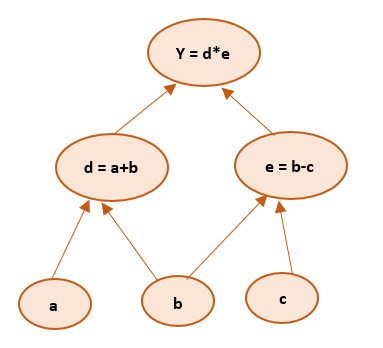
\includegraphics{../computation_graph.png}

Claim: \textit{functions described by computation graph are more general than normal pure functions in programming langauges}.

Here normal means the body of the function definitions is upper bounded, say by 30 lines (3 lines would be ideal for clean code).

\begin{rmk}
In Rust, there is a library called "salsa" where one can express the computation graph efficiently with memoization and value sharing. However, one needs to use macro and still need to keep track of many things.
\end{rmk}

\subsection{Pattern Recognition Graph}

\subsection{Modular Pattern Recognition Graph}

Pattern recognition graph is a specialized computational graph such that it's computable, learnable, explainable and well-suited to a specific domain.

(Explainability is possible because we only allow nodes to be associated with explainably types, i.e. a type such that the value of that type has clear meaning)

To avoid unnecessary confusion from over abstraction, we discuss computer vision and natural language separately, but the similarity can still be easy to see.

\begin{defn}[Pattern Recognition Graph for Image Input]
	The input is 2D rasterized image, i.e. a $M\times N$ matrix with each entry being RGB value.
\end{defn}

\subsection{Evolving Modular Pattern Recognition Graph}

\subsection {Expressive Power}

\subsubsection{Relational Database Query}


\subsubsection{Type Checking}

\subsubsection{Formal Verification and Theorem Proving}

\subsection{Transpilation to Neural Networks}

\subsection{Transpilation to More Efficient and Robustness Programs}

\end{document}